\section{Logarithmic scale}

\subsection{In human perception}

Logarithmic scale is very natural to human perceptions, including eyes.
When you ask average human to judge on current lighting, he/she may use words like ``dark'', ``very dark'', ``normal'', ``twilight'', ``bright'', 
``like on beach''.
In human language, there are couple of steps between ``dark'' and ``bright'', but luminous intensity may differ by several orders of magnitude.
Old cheap ``point-n-shoot'' photo cameras also has scale expressed in natural human languages.
But professional photo cameras also has logarithmic scales:

\begin{figure}[H]
\centering
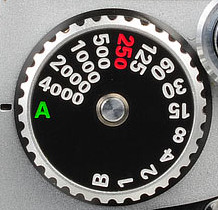
\includegraphics[scale=0.66]{log/nikon.jpg}
\caption{Shutter speed ($\frac{1}{x}$ of second) knob on photo camera}
\end{figure}

Another logarithmic scale familiar to anyone is decibel.
Even on cheap mp3 players and smartphones, where the volume is measured in conventional percents, this scale is logarithmic, 
and the difference between 50\% and 60\% may be much larger in sound pressure terms.

Yet another familiar to anyone logarithmic scale is Richter magnitude scale
\footnote{\url{https://en.wikipedia.org/wiki/Richter_magnitude_scale}}.
The Richter scale is practical, because when people talk about earthquakes, they are not interesting in exact scientific values
(in Joules or TNT equivalent), they are interesting in how bad damage is.

\subsection{In electronics engineering}

The loudspeakers are not perfect, so its output is non-linear in relation to input frequency.
In other word, loudspeaker has different loudness at different frequency.
It can be measured easily, and here is an example of plot of some speaker, I took it there:
\url{http://www.3dnews.ru/270838/page-3.html}.

\begin{figure}[H]
\centering
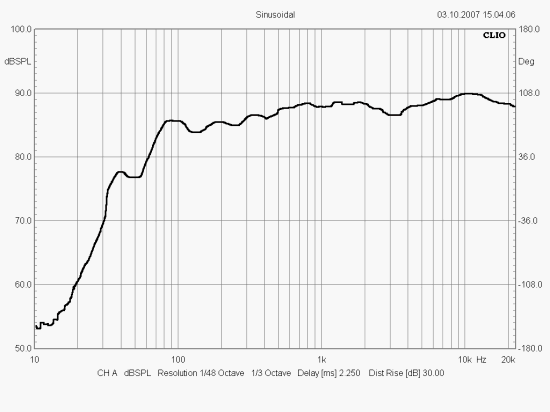
\includegraphics[scale=0.66]{log/65366.png}
\caption{Frequency response (also known as \textit{Bode plot}) of some loudspeaker}
\end{figure}

Both axis on this plot are logarithmic: y axis is loudness in decibel and x axis is frequency in Hertz.
Needless to say, the typical loudspeaker has bass/medium speaker + tweeter (high frequency speaker).
Some of more advanced loudspeaker has 3 speakers: bass, medium and tweeter.
Or even more.
And since the plot is logarithmic, each of these 2 or 3 speakers has their own part of plot, and these parts has comparable size.
If the x axis would be linear instead of logarithmic, the main part of it would be occupied by frequency response of tweeter alone, 
because it has widest frequency range. While bass speaker has narrowest frequency range, it would have very thin part of the plot.

y axis (vertical) of the plot is also logarithmic (its value is shown in decibels).
If this axis would be linear, the main part of it would be occupied by very loud levels of sound, while there would be thinnest line at the bottom
reserved for normal and quiet level of sounds.

Both of that would make plot unusable and impractical.
So both axis has logarithmic scale.
In strict mathematics terms, the plot shown is called \textit{log-log plot}, which means that both axis has logarithmic scale.

Summarizing, both electronics engineers and HiFi audio enthusiasts use these plots to compare quality of speakers.
These plots are often used in loudspeakers reviews
\footnote{Some of speakers of USSR era (like Latvian Radiotehnika S-30 and S-90) 
had such plots right on the surface of speaker box, presumably, for marketing purposes.}.

\subsection{In IT}

git, like any other VCS, can show a graph, how many changes each file got in each commit, for example:

\lstinputlisting{log/git_log.txt}

This scale is not logarithmical (I had a look into git internals), but this is exact place where logarithmical scale can be used.
When software developer got such report, he/she don't interesting in exact numbers of lines changed/added/removed.
He/she wants to see an outlook: which files got most changes/additions/removals, and which got less.

There is also a constraint: the space on the terminal is limited, so it's not possible to draw a minus or plus sign for each changed line of code.

Another example is Bitcoin client ``signal reception strength'', apparently, modeled after mobile phone signal indicator:

\begin{figure}[H]
\centering

\includegraphics[scale=1]{log/bitcoin_bars.png}
\caption{Bitcoin client}
\end{figure}

These bars indicating, how many connections client currently has.
Let's imagine, client can support up to 1000 connections, but user is never interesting in precise number, all he/she wants to know is how good its link
with Bitcoin network is.
I don't know how Bitcoin calculates this, but I think one bar could indicate that client has only 1 connection, two bars --- 2-5, three bars --- up to 10-20,
and four bars --- anything bigger.
This is also logarithmic scale.
On contrary, if you divide 1000 by 4 even parts, and one bar will fired if you've got 250 connections, two bars if you've got 500, etc, 
this would make the indicator useless, such indicators are no better than simple ``on/off'' lamp.

\subsection{Web 2.0}

Sites like GitHub, Reddit, Twitter sometimes shows how long some event was ago, instead of precise date (at least in 2015).
For example, Reddit may show date as ``3 years ago'', ``11 months ago'', ``3 weeks ago'', ``1 day ago'', ``10 hours ago'', etc, down to minutes and seconds.
You wouldn't see ``3 years and 11 hours ago''.
This is also logarithmic scale.
When some event happens 10 months ago, users are typically not interesting in precision down to days and hours.
When something happens 2 years ago, users usually not interesting in number of months and days in addition to these 2 years.

